\chapter{Edge Detection}

As mentioned earlier, road detection is performed in squares of 32 px. When determining the exact transition from road to non-road, the best possible accuracy is 32 px. To determine the precise transition from road to non-road, edge detection will be used. It can also be used as fallback when the road detection fails.
\npar 
\subsection{Removing details}

Detecting edges is very straightforward using an edge detection algorithm like Canny Edge Detection \cite{canny}. However, there are a lot of edges on the road itself, thinking of road markings and cobbles. The edges on the road, considered as noise, and the edges of the road are not unambiguously separable. The width of the patterns that cause the edges on the road is rather small. Using morphological image processing operations, it is possible to remove these small patterns.  In figure \ref{cobbles_erode_out}, a smoothed cobbled road is shown.
\begin{figure}[ht]
\centering
\begin{subfigure}{.5\textwidth}
  \centering
  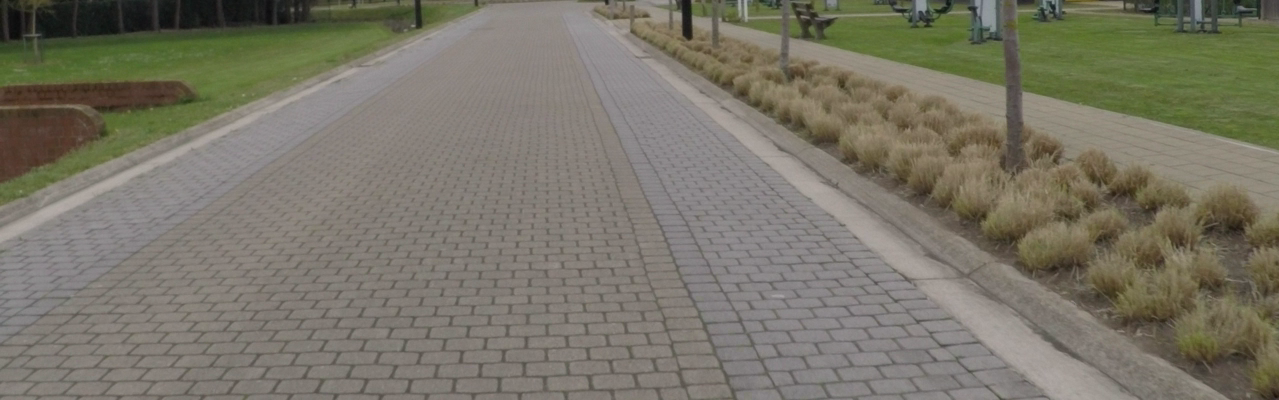
\includegraphics[width=.9\textwidth]{cobbles_in}
  \caption{Original frame\label{cobbles_in}}
\end{subfigure}%
\begin{subfigure}{.5\textwidth}
  \centering
  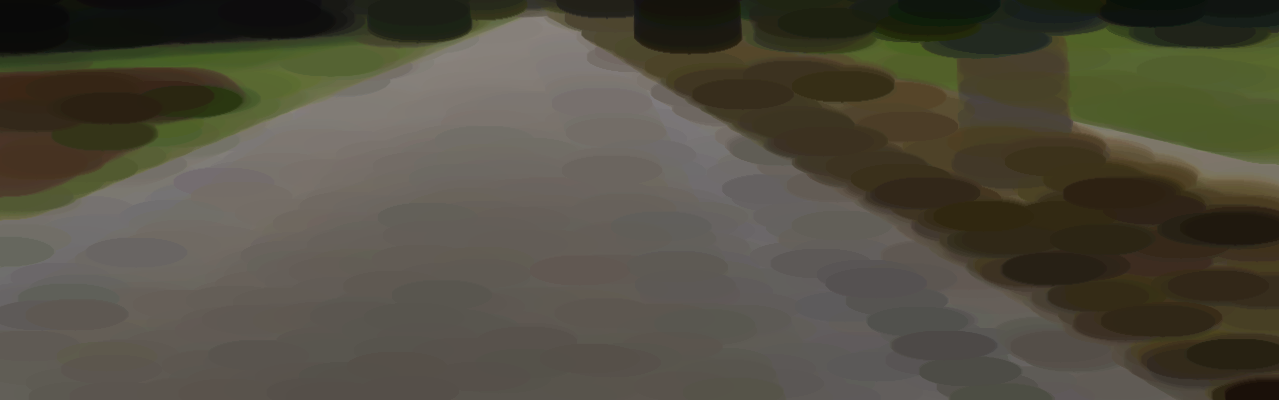
\includegraphics[width=.9\textwidth]{cobbles_erode_out}
  \caption{Eroded cobbled road\label{cobbles_erode_out}}
\end{subfigure}
\caption{Perform eroding to remove the edges on the road.}
\end{figure}


\npar
Eroding is a morphology operator to make the objects on the foreground, which are the brightest, smaller \cite{erode_dilate}. Figure \ref{line_zoom_eroded} shows an example of a thinned white line. When the kernel is large enough, white lines can be filtered out completely. The same technique is used to smooth the surface of cobbled roads. A cobblestone consist of a bright center, surrounded by darker joints. By eroding the cobbled road, the erode function will minimize the center of the cobble, which will cause enlarged joints. With a large kernel, the joints will spread until they overlap. The best results were achieved with an ellipsoidal kernel of 100 x 30 px.

\begin{figure}[ht]
	\begin{minipage}[t]{.45\textwidth}
		\centering
		\begin{subfigure}[t]{.5\textwidth}
		  \centering
		  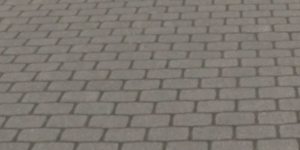
\includegraphics[width=.9\textwidth]{cobbles_zoom_original}
		  \caption{Original frame\label{cobbles_zoom_original}}
		\end{subfigure}%
		\begin{subfigure}[t]{.5\textwidth}
		  \centering
		  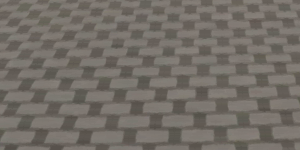
\includegraphics[width=.9\textwidth]{cobbles_zoom_eroded}
		  \caption{Bigger joints after eroding\label{cobbles_zoom_eroded}}
		\end{subfigure}
		\caption{The effect of eroding cobbled roads.}
	\end{minipage}%
	\hspace{0.05\textwidth}
	\begin{minipage}[t]{.45\textwidth}
		\centering
		\begin{subfigure}[t]{.5\textwidth}
		  \centering
		  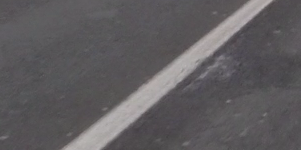
\includegraphics[width=.9\textwidth]{line_zoom_original}
		  \caption{Original frame\label{line_zoom_original}}
		\end{subfigure}%
		\begin{subfigure}[t]{.5\textwidth}
		  \centering
		  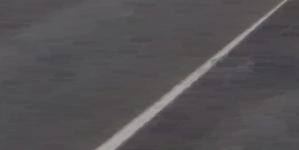
\includegraphics[width=.9\textwidth]{line_zoom_eroded}
		  \caption{Smaller lines after eroding\label{line_zoom_eroded}}
		\end{subfigure}
		\caption{The effect of eroding road markings.}
	\end{minipage}
\end{figure}

\npar
Unfortunately, the erode function will cause the darker objects to expand. The original size of the objects has been modified, as seen in \ref{car_erode_bigger}. This will falsify the eventual edge detection. In this example, the observed car is reported to close. In order to restore the original measures, dilation is executed. This is the opposite morphology operator of eroding. The combination of eroding and dilation is called opening. When dilation is executed with the same kernel size of the erode function, the original size of the dark objects will decrease to their original size, as seen in \ref{car_dilate_smaller}. Note that, after eroding, some details of the shape of the objects are lost. In order to provide a safety margin, the dilate function is executed with a slightly smaller kernel.


\begin{figure}[ht]
\centering
\begin{subfigure}{.5\textwidth}
  \centering
  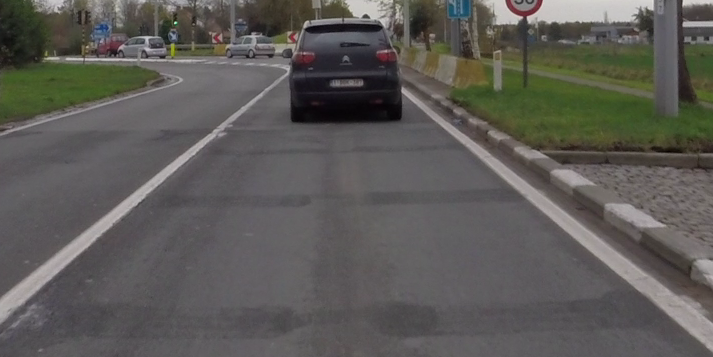
\includegraphics[width=.9\textwidth]{car_original}
  \caption{Original frame\label{car_original}}
\end{subfigure}%
\begin{subfigure}{.5\textwidth}
  \centering
  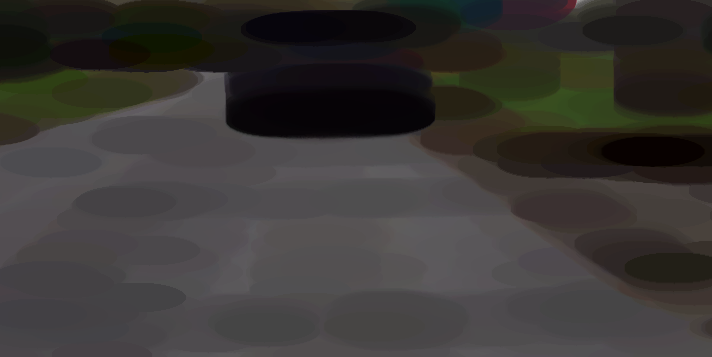
\includegraphics[width=.9\textwidth]{car_erode_bigger}
  \caption{Dark objects are bigger after eroding\label{car_erode_bigger}}
\end{subfigure}
\begin{subfigure}{.5\textwidth}
  \centering
  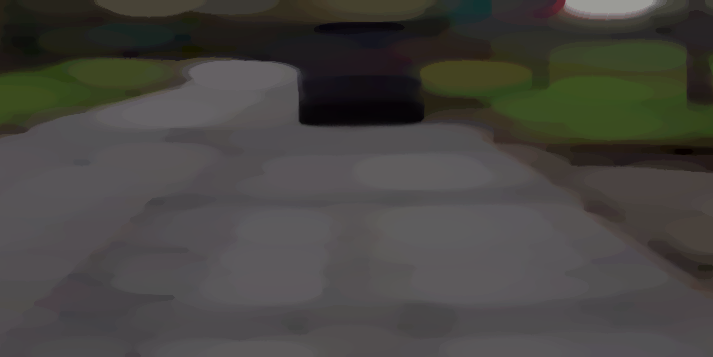
\includegraphics[width=.9\textwidth]{car_dilate_smaller}
  \caption{Restore original sizes with dilation\label{car_dilate_smaller}}
\end{subfigure}
\caption{Perform eroding and dilation to remove details.}
\end{figure}

\subsection{Canny Edge Detection}

To detect the edges of the road, the Canny Edge Detection algorithm is used. Figure \ref{canny_edges} shows an example. 


\begin{figure}[ht]
	\centering
	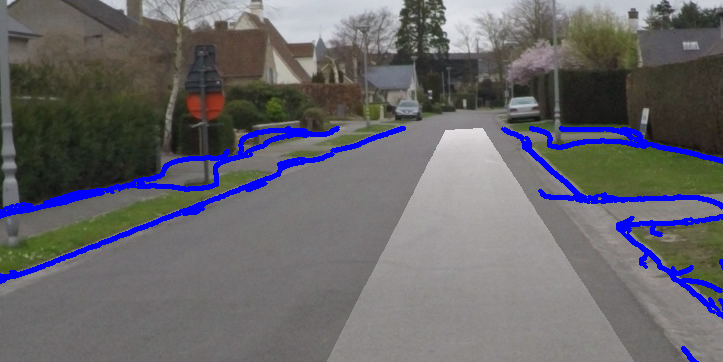
\includegraphics[width=.5\textwidth]{canny_edges}
	\caption{Canny edge detection\label{canny_edges}}
\end{figure}


\npar
This algorithm requires a minimum and a maximum threshold value, which were determined experimentally. 
The best results were achieved with a maximum threshold that is twice the minimum threshold.
The minimum threshold is determined by the required minimum sensitivity. When the algorithm is configured too sensitive, some imperfections on the road will be detected as edges. On the other hand, a certain level of sensitivity is necessary to detect less clear road edges. For example, a transition from road to dirt has a very small distinction of color and brightness, as seen in \ref{transition_road_dirt_eroded}. The minimum threshold should be high enough to detect this transition as edge. 

\begin{figure}[ht]
\centering
\begin{subfigure}{.5\textwidth}
  \centering
  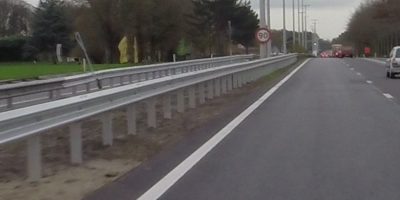
\includegraphics[width=.9\textwidth]{transition_road_dirt_original}
  \caption{Original frame\label{transition_road_dirt_original}}
\end{subfigure}%
\begin{subfigure}{.5\textwidth}
  \centering
  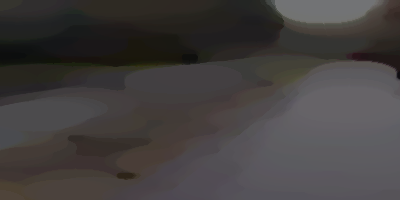
\includegraphics[width=.9\textwidth]{transition_road_dirt_eroded}
  \caption{Eroded road\label{transition_road_dirt_eroded}}
\end{subfigure}
\caption{Unclear transition from road to non-road.}
\end{figure}

